\documentclass{beamer}
\usepackage{ChaosConsultingStil}
\usepackage{listings}
\usepackage{color}
%lstlisting Einstellungen 
\definecolor{light-gray}{gray}{0.95}
\lstset{ 
basicstyle=\scriptsize\tt,
backgroundcolor=\color{light-gray},
}
\begin{document}
\title[Smartcards unter Linux]{Smartcards unter Linux}
\subtitle[Praktische Anwendungsfälle]{Praktische Anwendungsfälle}
\author[domfi]{Dominik Fischer}
\date{2016-01-09}
\institute[Chaos Consulting e.V.]{\vspace{0.5cm}\includegraphics[scale=0.5]{cc_header.png}}

\begin{frame}
\titlepage	
\end{frame}
\begin{frame}{Inhaltsverzeichnis}
	\tableofcontents
\end{frame}

\section{Grundlagen}
%\begin{frame}{Was sind Smartcards?}
%\begin{minipage}[t][\textheight][t]{\linewidth}
%\begin{itemize}
%	\item Chipkarten mit Microprozessor, RAM, ROM, EEPROM 
%	\item Punkt 2
%\end{itemize}
%\end{minipage}
%\end{frame}

\begin{frame}{HW-Komponenten: Smartcard}
Smartcards \emph{(ICC -- integrated circuit card)} gibt es vielen Ausführungen.
Sie unterscheiden sich in folgenden Punkten:
\vspace{10mm}
\begin{columns}
\begin{column}{0.5\textwidth}
\begin{minipage}[t][\textheight][t]{\linewidth}
\begin{itemize}
  \item Format: ID-1 (EC-Karte), ID-000 (normale SIM-Karten), \ldots
  \item kontaktbehaftet / kontaktlos
  \item Betriebssysteme 
\end{itemize}
\end{minipage}
\end{column}
\begin{column}{0.5\textwidth}
\begin{minipage}[t][\textheight][t]{\linewidth}
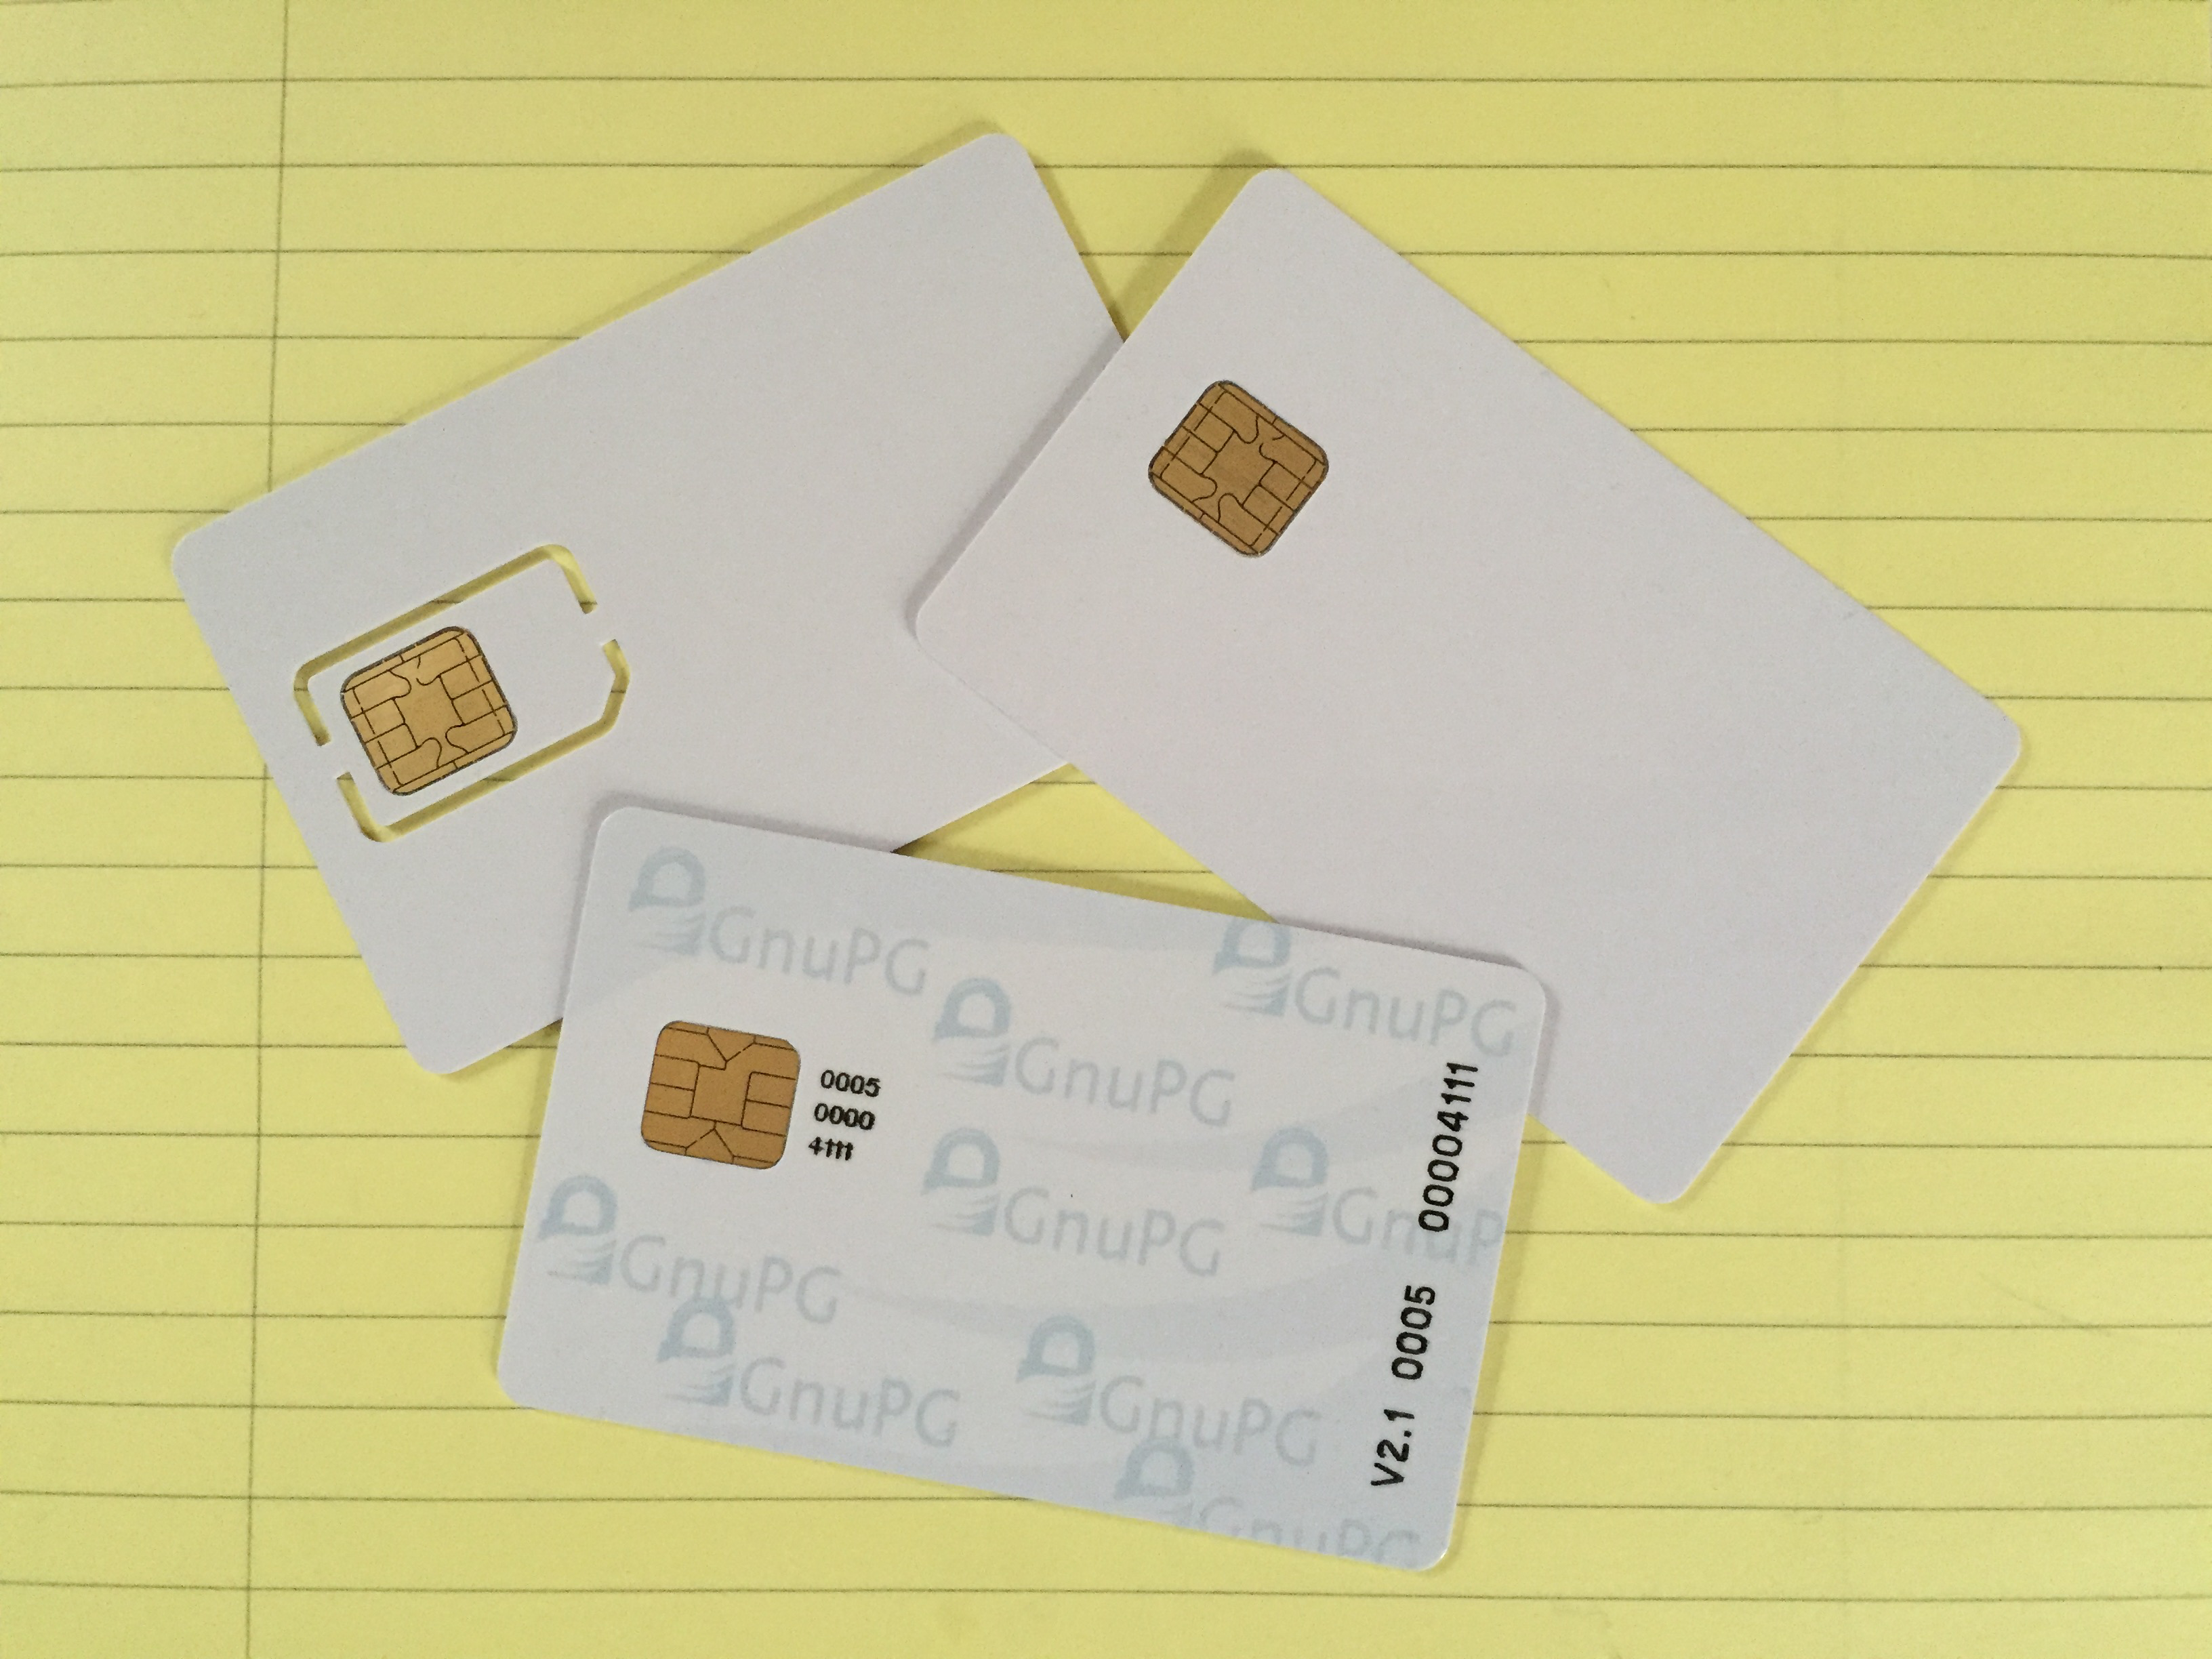
\includegraphics[width=\columnwidth]{smartcards.png}
\end{minipage}
\end{column}
\end{columns}
\end{frame}

\begin{frame}[fragile]{Speicherorganisation}
\begin{minipage}[t][\textheight][t]{\linewidth}
\begin{itemize}
  \item ROM (Betriebssystem), RAM (Arbeitsdaten), EEPROM (Dateisystem)
  \item Dateisystem (standardisiert in ISO 7816-4)
  \begin{itemize}
    \item MF (master file): Root-Verzeichnis
    \item DF (dedicated file): Verzeichnisdateien
    \item EF (elementary file): Nutzdaten
    \item Inhalt durschstöbern z.B. mit: \lstinline|opensc-browser|
  \end{itemize}
\end{itemize}
\end{minipage}
\end{frame}

\begin{frame}{HW-Komponenten: Smartcard-Reader}
Smartcardleser \emph{(IFD -- interface device}) werden gemäß
ihrer Sicherheit in drei Klassen unterteilt.
\vspace{10mm}
\begin{columns}
\begin{column}{0.5\textwidth}
\begin{minipage}[t][\textheight][t]{\linewidth}
\begin{itemize}
  \item Class-1: Nur Kontakteinheit
  \item Class-2: Kontakteinheit mit Tastatur zur PIN-Eingabe
  \item Class-3: Kontakteinheit mit Tastatur und Display
\end{itemize}
\end{minipage}
\end{column}
\begin{column}{0.5\textwidth}
\begin{minipage}[t][\textheight][t]{\linewidth}
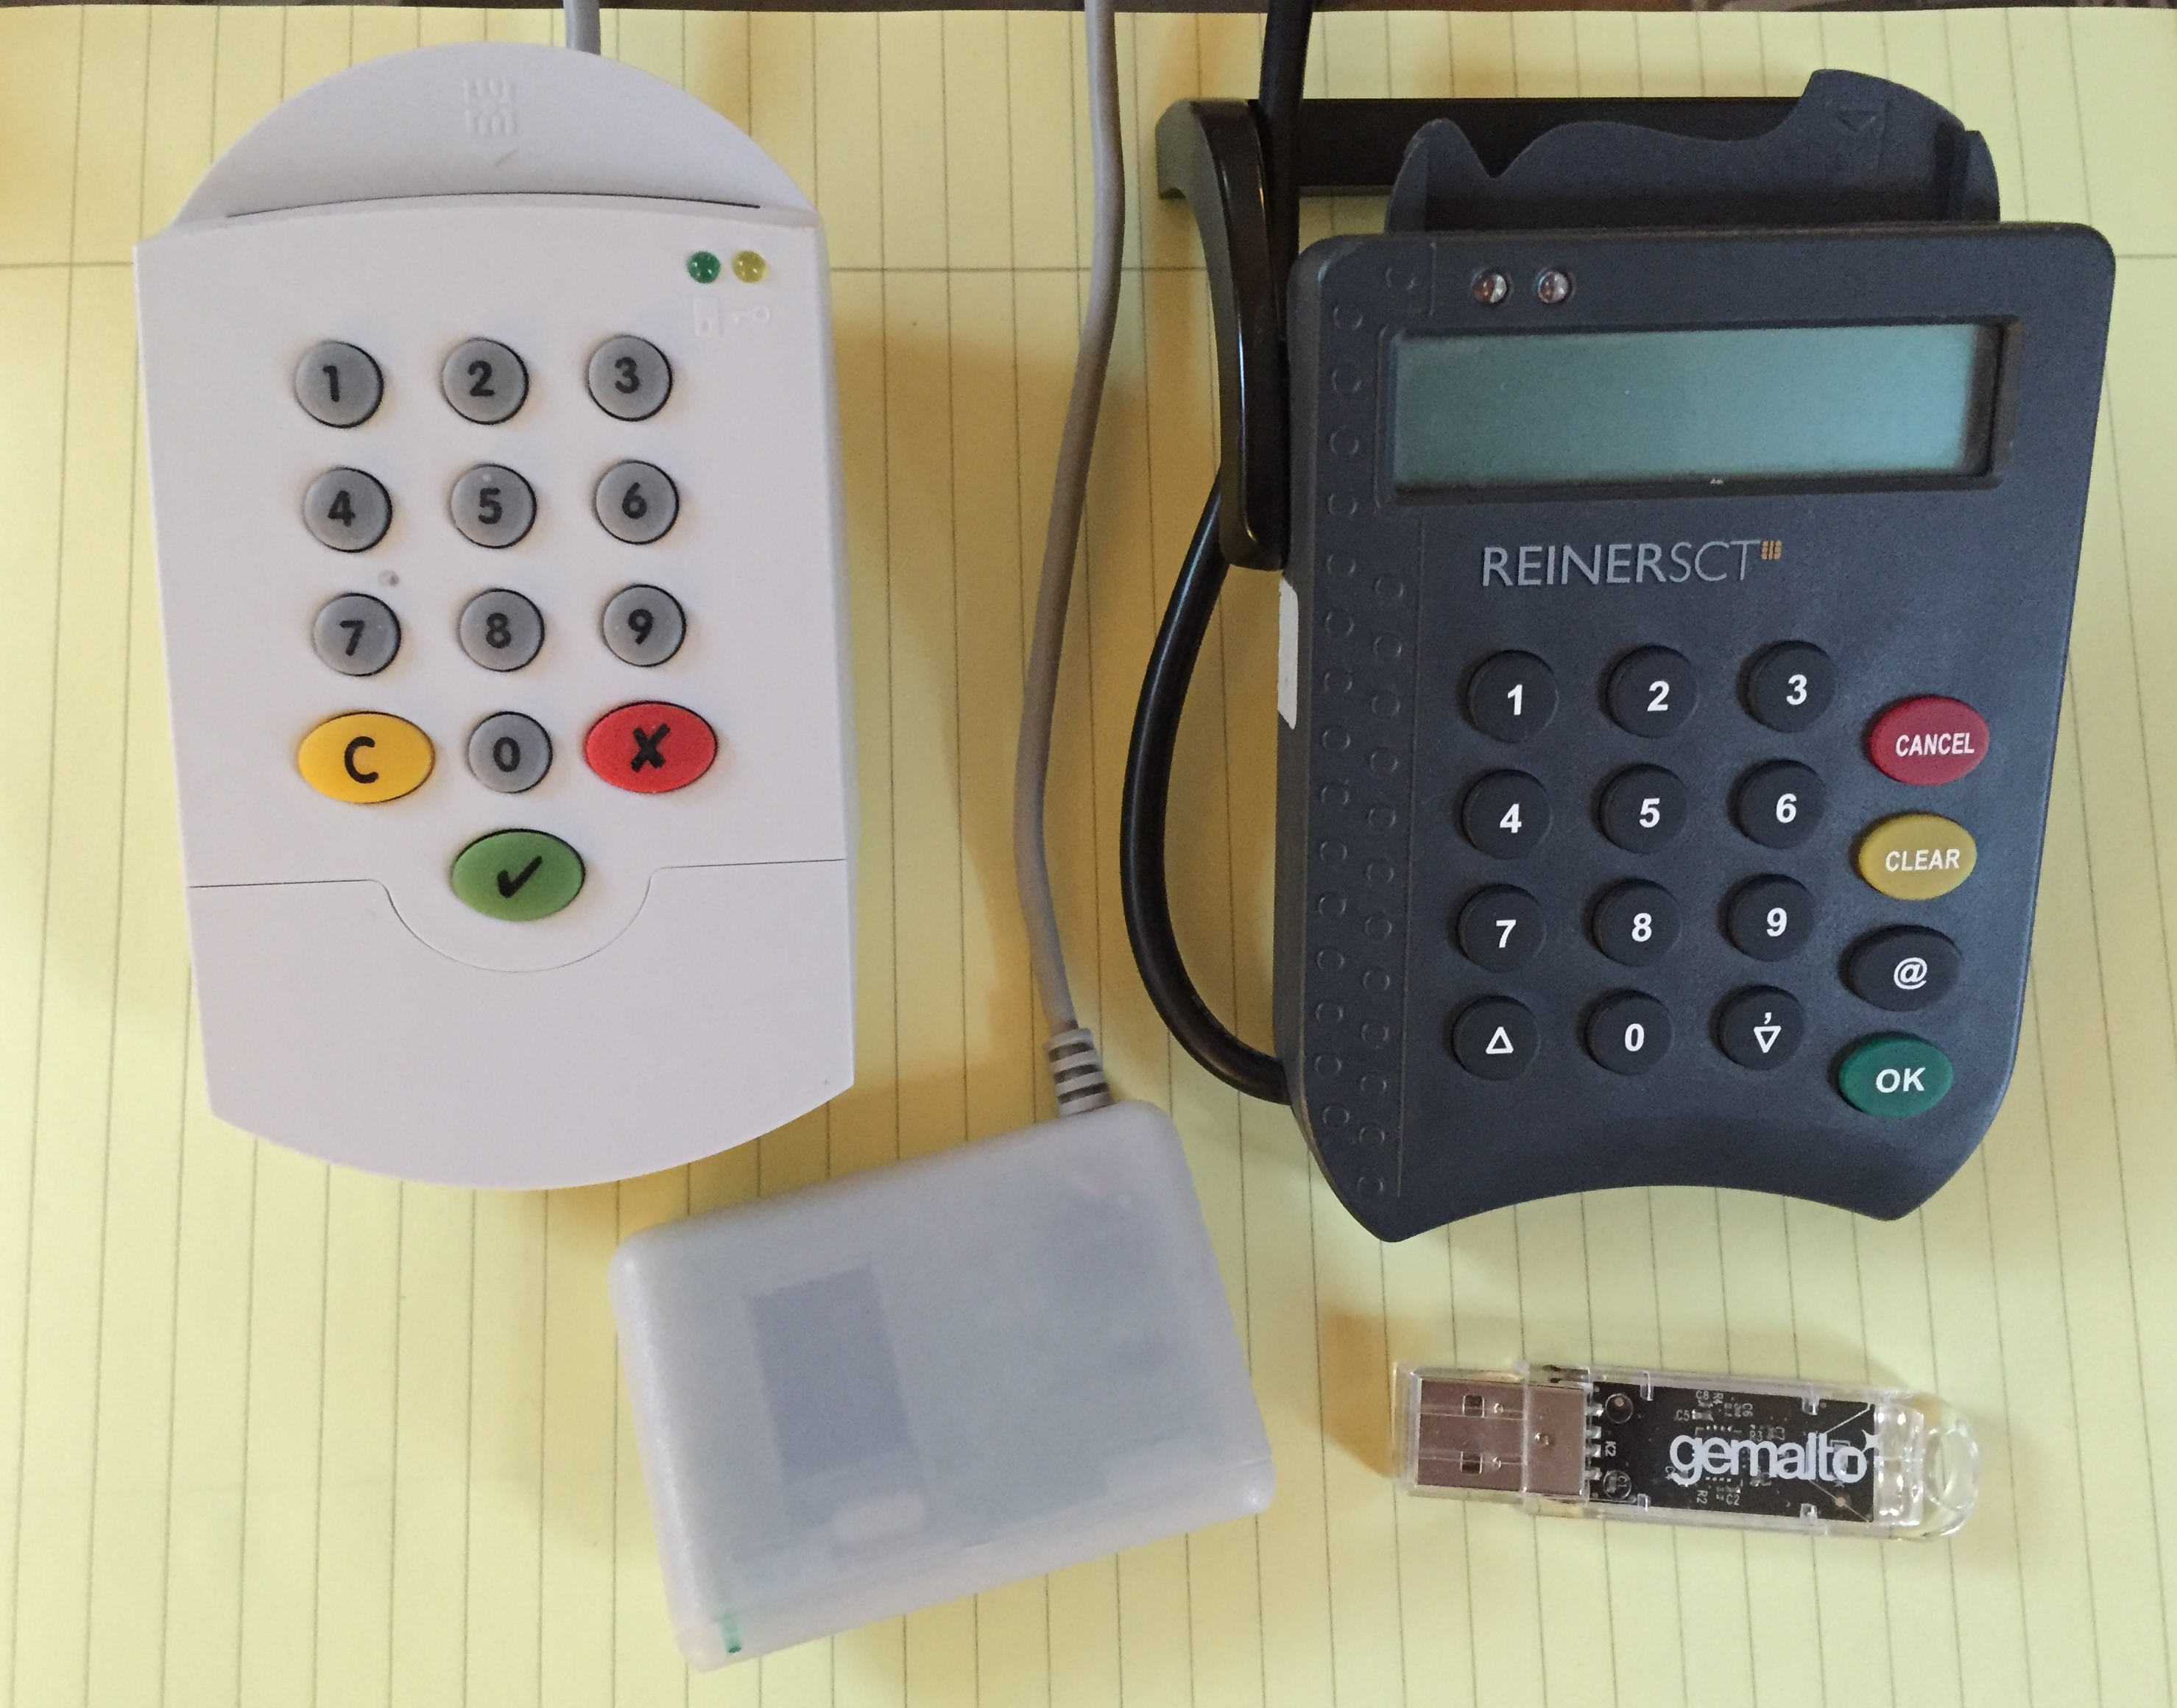
\includegraphics[width=\columnwidth]{reader.png}
\end{minipage}
\end{column}
\end{columns}
\end{frame}

\begin{frame}[fragile]{Softwarekomponenten}
Benötigte Softwarekomponenten installieren:
\begin{itemize}
  \item Gerätetreiber
  \item API für Low-Level Zugriff:
  \begin{itemize}
    \item OCF (open card framework)
    \item PC/SC (personal computer/smart card)
  \end{itemize}
  \item Crypto-API
\end{itemize}

\begin{lstlisting}
$ sudo apt-get install \
    libccid pcscd \
    opensc opensc-pkcs11
\end{lstlisting}
\end{frame}

\begin{frame}[fragile]{Ersten Schritte: opensc-tool}
\begin{minipage}[t][\textheight][t]{\linewidth}
\begin{itemize}
  \item Erkannte Reader auflisten: 
  \begin{lstlisting}
# opensc-tool -l
# Detected readers (pcsc)
Nr. Card Features  Name
0   Yes            Gemalto GemPC Express(...)
  \end{lstlisting}
  \item ATR der Karte auflisten
  \begin{lstlisting}
# opensc-tool -r 0 -a
3b:fe:18:00:00:81:31:fe:45:80:31:81:54:48(...)  
  \end{lstlisting}
  \item Karte identifizieren
  \begin{lstlisting}
# opensc-tool -r 0 -n
SmartCard-HSM
  \end{lstlisting}
  \item Dateien auf der Karte auflisten
  \begin{lstlisting}
# opensc-tool -r 0 -f
3f00 type: DF, size: 0
(...)
  \end{lstlisting}
\end{itemize}
\end{minipage}
\end{frame}

\begin{frame}[fragile]{Smartcard initialisieren: pkcs15-init}
\begin{minipage}[t][\textheight][t]{\linewidth}
Normalerweise wird \lstinline|pkcs15-init| benutzt, aber bei dem hier
verwendeten Smartcard-Typ funktioniert das nicht. Stattdessen muss das Tool
\lstinline|sc-hsm-tool| verwendet werden.
\begin{itemize}
  \item SO-PIN: genau 16 hexadezimale Ziffern
  \item User-Pin: 6 bis 16 ASCII-Zeichen, kann
geändert werden, aber nicht die Länge  (dafür muss man reinitialisieren und
alles Löschen)
\end{itemize}
\begin{lstlisting}
# sc-hsm-tool --initialize \
    --so-pin 0123012301230123 \
    --pin 123456 \
    --label Chaosconsulting
\end{lstlisting}
\end{minipage}
\end{frame}

\begin{frame}[fragile]{Objekte anschauen: pkcs15-tool}
\begin{minipage}[t][\textheight][t]{\linewidth}
\begin{itemize}
  \item Objekte der Karte dumpen
\end{itemize}
\begin{lstlisting}
# pkcs15-tool -D
Using reader with a card: Gemalto GemPC Express 00 00
PKCS#15 Card [Chaosconsulting]:
  Version        : 0
  Serial number  : DECM0102470
  Manufacturer ID: www.CardContact.de
  Flags          : PRN generation

PIN [UserPIN]
  Object Flags   : [0x3], private, modifiable
  (...)

PIN [SOPIN]
  Object Flags   : [0x1], private
  (...)
\end{lstlisting}
\end{minipage}
\end{frame}

\begin{frame}[fragile]{Schlüsselpaar erzeugen: pkcs11-tool}
\begin{minipage}[t][\textheight][t]{\linewidth}
\begin{lstlisting}
# pkcs11-tool -l --keypairgen \
    --key-type rsa:2048 \
    --id 10 \
    --label "My first RSA keypair"
    
Using slot 1 with a present token (0x1)
Logging in to "Chaosconsulting (UserPIN)".
Please enter User PIN: 
Key pair generated:
Private Key Object; RSA 
  label:      My first RSA keypair
  ID:         10
  Usage:      decrypt, sign, unwrap
Public Key Object; RSA 2048 bits
  label:      My first RSA keypair
  ID:         10
  Usage:      encrypt, verify, wrap

\end{lstlisting}
\end{minipage}
\end{frame}

\begin{frame}[fragile]{Dateien verschlüsseln}
\begin{minipage}[t][\textheight][t]{\linewidth}
\begin{itemize}
  \item \emph{PublicKey} auslesen
\begin{lstlisting}
$ pkcs15-tool --read-public-key 10 > pubkey.pem
$ echo "Hallo Welt!" > foobar.txt
$ sha256sum foobar.txt
1cf0c75265e678c4b9bcc32a798e8d484b (...)
\end{lstlisting}
  \item Datei mit \emph{PublicKey} verschlüsseln
\begin{lstlisting}
$ openssl rsautl -inkey pubkey.pem \
    -pubin -encrypt -pkcs -in foobar.txt \
    -out foobar.txt.encrypted
$ sha256sum foobar.txt.encrypted
fbc38a86a60c500aab1251ec1110d41ebe (...)
\end{lstlisting}
  \item Datei mit {PrivateKey} von Smartcard entschlüsseln
\begin{lstlisting}
$ pkcs15-crypt --decipher --key 10 \
    --input foobar.txt.encrypted \
    --pkcs1 --raw > foobar.txt.encrypted.decrypted
$ sha256sum foobar.txt.encrypted.decrypted
1cf0c75265e678c4b9bcc32a798e8d48 (...)
\end{lstlisting}
\end{itemize}
\end{minipage}
\end{frame}

\section{SSH}

\begin{frame}[fragile]{Smartcardverschlüsselte SSH-Verbindung}
\begin{minipage}[t][\textheight][t]{\linewidth}
\begin{itemize}
	\item Public-Key im SSH-Format ausgeben
	\begin{lstlisting}
$ pkcs15-tool --read-ssh-key 10
Using reader with a card: Gemalto GemPC Express 00 00
ssh-rsa AAAAB3NzaC1yc2EAAAADAQABAAABAQDI0TlV (...)
	\end{lstlisting}
	\item Der \emph{PublicKey} muss in die \lstinline|~/.ssh/authorized_keys|
	auf dem entfernten Host eingetragen werden
	\item Smartcard mit SSH verwenden. Als Identity-File wird die PKCS\#11 Library
	angegeben.
	\begin{lstlisting}
$ ssh -I /usr/lib/x86_64-linux-gnu/opensc-pkcs11.so \
    user@entfernter.host 
Enter PIN for 'Chaosconsulting (UserPIN)': 
	\end{lstlisting}
\end{itemize}
\end{minipage}
\end{frame}

\begin{frame}[fragile]{Bequemer mit ssh-agent}
\begin{minipage}[t][\textheight][t]{\linewidth}
\begin{itemize}
  \item Der \lstinline|ssh-agent| wird auf den meisten Linux-Systemen
  automatisch beim Login gestartet
  \item Der \lstinline|gnome-keyring-daemon| darf nicht dazwischen kommen!
  \item Token zum SSH-Agenten hinzufügen
  \begin{lstlisting}
$ ssh-add -s /usr/lib/x86_64-linux-gnu/opensc-pkcs11.so
  \end{lstlisting}
  \item Vom ssh-agent verwaltete Schlüssel anzeigen
  \begin{lstlisting}
$ ssh-add -l
  \end{lstlisting}
  \item Token vom SSH-Agenten entfernen
  \begin{lstlisting}
$ ssh-add -e /usr/lib/x86_64-linux-gnu/opensc-pkcs11.so
  \end{lstlisting}
\end{itemize}
\end{minipage}
\end{frame}

\section{Login mit PAM}

\begin{frame}[fragile]{pam\_pkcs11 einrichten}
\begin{minipage}[t][\textheight][t]{\linewidth}
\begin{itemize}
	\item Nötige Pakete installieren
	\begin{lstlisting}
# apt-get install libpam-pkcs11 libengine-pkcs11-openssl
	\end{lstlisting}
   \item Konfiguration \lstinline|/etc/pam_pkcs11/pam_pkcs11.conf| anlegen
\begin{lstlisting}[basicstyle=\tiny\tt]
$ cp /usr/share/doc/libpam-pkcs11/examples/pam_pkcs11.conf.example \
    /etc/pam_pkcs11/pam_pkcs11.conf
$ vi /etc/pam_pkcs11/pam_pkcs11.conf
pam_pkcs11 {
 (...)
 use_pkcs11_module = opensc;
 pkcs11_module opensc {
  module = /usr/lib/x86_64-linux-gnu/opensc-pkcs11.so;
  (...)
 }
 use_mappers = openssh;
 (...)
}
\end{lstlisting}
\end{itemize}
\end{minipage}
\end{frame}

\begin{frame}[fragile]{PAM konfigurieren}
\begin{minipage}[t][\textheight][t]{\linewidth}
Für den PAM Typ \emph{auth} muss das pam\_pkcs11 Modul bei den
gewünschten Services eingetragen werden. 

Z.B. für Logins in der  Datei \lstinline|/etc/pam.d/sudo|:
\begin{lstlisting}
auth       sufficient    pam_pkcs11.so nullok try_first_pass 
(...)
\end{lstlisting}
Ähnliche Einträge werden bei den anderen Diensten vorgenommen
(z.B. für das grafische Login, sudo, screensaver, etc.).

\vspace{10mm}

\colorbox{yellow}{!!! Vorsicht bei der Anpassung von PAM !!!}

Vorher immer mehrere Logins mit Root-Sessions öffnen \\
und gut testen, damit man sich nicht aussperrt!!!

\end{minipage}
\end{frame}

\begin{frame}[fragile]{X.509 Zertifikat erstellen}
\begin{minipage}[t][\textheight][t]{\linewidth}
\begin{itemize}
	\item Nötige Pakete installieren
	\begin{lstlisting}
\# apt-get install libpam-pkcs11 libengine-pkcs11-openssl
	\end{lstlisting}
	\item Zertifikat erstellen
	\begin{lstlisting}
$ openssl
# Engine einrichten...
OpenSSL> engine -t dynamic \
  -pre SO_PATH:/usr/lib/engines/engine_pkcs11.so
  -pre ID:pkcs11 -pre LIST_ADD:1 -pre LOAD \
  -pre MODULE_PATH:/usr/lib/x86_64-linux-gnu/opensc-pkcs11.so

# Certificate Signing Request erstellen...
OpenSSL> req -engine pkcs11 -new -key 1:10 \
  -keyform engine -out req.pem
  -text -x509 -subj "/CN=Dominik Fischer"

# Zertifikat ausstellen...
OpenSSL> x509 -engine pkcs11 -signkey 1:10 \
  -keyform engine -in req.pem -out cert.pem
    \end{lstlisting}
\end{itemize}
\end{minipage}
\end{frame}

\begin{frame}[fragile]{X.509 Zertifikat erstellen \(continued\)}
\begin{minipage}[t][\textheight][t]{\linewidth}
\begin{itemize}
	\item Dateiformat umwandeln
	\begin{lstlisting}
$ openssl x509 -in cert.pem -out cert.der -outform der	
	\end{lstlisting}
	\item Zertifikat auf Smartcard schreiben
	\begin{lstlisting}
$ pkcs11-tool \
    --module /usr/lib/x86_64-linux-gnu/opensc-pkcs11.so \ 
    -l --write-object cert.pem \
    --type cert \
    --id 45 --label "MyCert"
	\end{lstlisting}
\end{itemize}
\end{minipage}
\end{frame}

\begin{frame}[fragile]{Login für einen Account erlauben}
\begin{minipage}[t][\textheight][t]{\linewidth}
\begin{itemize}
  \item Da wir den openssh Mapper beim pam\_pkcs11 ausgewählt haben, Wie zuvor
  bei SSH: Key im SSH Format auslesen und in die \lstinline|authorized\_keys|
  des Accounts eintragen.
\end{itemize}
\begin{lstlisting}

\end{lstlisting}
\end{minipage}
\end{frame}

\section{GnuPG}
\begin{frame}[fragile]{OpenPGP Card und gnupg}
\begin{minipage}[t][\textheight][t]{\linewidth}
\begin{itemize}
	\item Die OpenPGP ist ähnlich wie die bisher besprochenen Karten. Sie hat eine
	vordefinierte Datenstruktur (\lstinline|pkcs15-tool -D| zeigt sie an).
	\item GnuPG hat Optionen zur Verwaltung der Karte
	\item Kartenstatus anzeigen:
	\begin{lstlisting}
$ gpg --card-status
gpg: detected reader `Gemalto GemPC Express 01 00'
Application ID ...: D2760001240102010005000041BC0000
Version ..........: 2.1
Manufacturer .....: ZeitControl
(...)	
	\end{lstlisting}
	\item Karteninhalt editieren:
	\begin{lstlisting}
$ gpg --card-edit
(...)
gpg/card> help
quit       Menü verlassen
admin      Zeige Admin-Befehle
(...)
	\end{lstlisting}
\end{itemize}
\end{minipage}
\end{frame}

\begin{frame}[fragile]{Dateien ver-/entschlüsseln}
\begin{minipage}[t][\textheight][t]{\linewidth}
\begin{itemize}
  \item Verschlüsseln
  \begin{lstlisting}
$ gpg -ea -r mmuster@example.com foobar.txt
  \end{lstlisting}
  \item Entschlüsseln
  \begin{lstlisting}
$ gpg -d --output foobar.txt.asc.decrypted foobar.txt.asc
  \end{lstlisting}
\end{itemize}
\end{minipage}
\end{frame}

\begin{frame}[fragile]{GnuPG Keyring wieder herstellen}
\begin{minipage}[t][\textheight][t]{\linewidth}
\begin{itemize}
  \item Public Key muss außerhalb der Karte gespeichert sein. Am einfachsten
  direkt nach der Erstellung auf einen Keyserver hochladen:
  \begin{lstlisting}
$ gpg --send-keys 6C7F8E30
  \end{lstlisting}
  \item Auf frischem Rechner ausführen:
  \begin{lstlisting}
$ gpg --list-keys
$ gpg --card-edit
gpg/card> fetch
  \end{lstlisting}
\end{itemize}
Damit wurden die nötigen Dateien unter \lstinline{~/.gnupg} erstellt.
\end{minipage}
\end{frame}

\section{Festplattenverschlüsselung}

\begin{frame}[fragile]{Festplattenverschlüsselung}
\begin{minipage}[t][\textheight][t]{\linewidth}
\begin{itemize}
  \item Die Verwendung von LUKS mit Smartcard ist möglich, wird hier allerdings
  nicht betrachtet.
  \item Veracrypt (Nachfolger von TrueCrypt) unterstützt PKCS\#11-Tokens und
  damit auch Smartcards.
\end{itemize}
\end{minipage}
\end{frame}

\begin{frame}[fragile]{Veracrypt}
\begin{minipage}[t][\textheight][t]{\linewidth}
\begin{itemize}
  \item Beim Anlegen des Volumes muss ein Keyfile erstellt werden
  \item Das Keyfile wird dann im Terminal per PIN geschützt als Objekt auf die
  Smartcard übertragen
  \item In den Veracrypt Einstellungen muss der Pfad zur opensc-pkcs11 Library
  eingetragen werden (Settings -- Preferences\ldots -- Security Token)
\end{itemize}
\end{minipage}
\end{frame}

\section{Links}
\begin{frame}[fragile]{Links}
\begin{minipage}[t][\textheight][t]{\linewidth}
\begin{itemize}
  \item Wikipedia zu Chipkarten: \url{https://de.wikipedia.org/wiki/Chipkarte}
  \item OpenPGP-Card: \url{http://shop.kernelconcepts.de}
  \item SmartCard-HSM: \url{http://www.cardomatic.de/}
  \item OpenSC Projekt: \url{https://github.com/OpenSC}
  \item PKCS:
  \url{https://de.wikipedia.org/wiki/Public-Key_Cryptography_Standards}
  \item Veracrypt: \url{https://veracrypt.codeplex.com/}
\end{itemize}
\end{minipage}
\end{frame}

\end{document}
